\RequirePackage{luatex85,shellesc}
\documentclass[crop,tikz]{standalone}
\usepackage{pgfplots}
\usepgfplotslibrary{fillbetween}
\usetikzlibrary{shapes,calc}
\usepackage{xcolor}

\definecolor{ncbsgreen}{rgb}{0.07,0.29,0.09}
\definecolor{ncbsred}{rgb}{0.20,0.40,0.11}
\definecolor{ncbstext}{rgb}{0.18,0.18,0.18}

\begin{document}

\def\drawcirculararc(#1,#2)(#3,#4)(#5,#6){%
        \pgfmathsetmacro\cA{(#1*#1+#2*#2-#3*#3-#4*#4)/2}%
        \pgfmathsetmacro\cB{(#1*#1+#2*#2-#5*#5-#6*#6)/2}%
        \pgfmathsetmacro\cy{(\cB*(#1-#3)-\cA*(#1-#5))/%
                            ((#2-#6)*(#1-#3)-(#2-#4)*(#1-#5))}%
        \pgfmathsetmacro\cx{(\cA-\cy*(#2-#4))/(#1-#3)}%
        \pgfmathsetmacro\cr{sqrt((#1-\cx)*(#1-\cx)+(#2-\cy)*(#2-\cy))}%
        \pgfmathsetmacro\cA{atan2(#1-\cx,#2-\cy)}%
        \pgfmathsetmacro\cB{atan2(#5-\cx,#6-\cy)}%
        \pgfmathparse{\cB<\cA}%
        \ifnum\pgfmathresult=1
                \pgfmathsetmacro\cB{\cB+360}%
        \fi
        \draw (#1,#2) arc (\cA:\cB:\cr);%
}

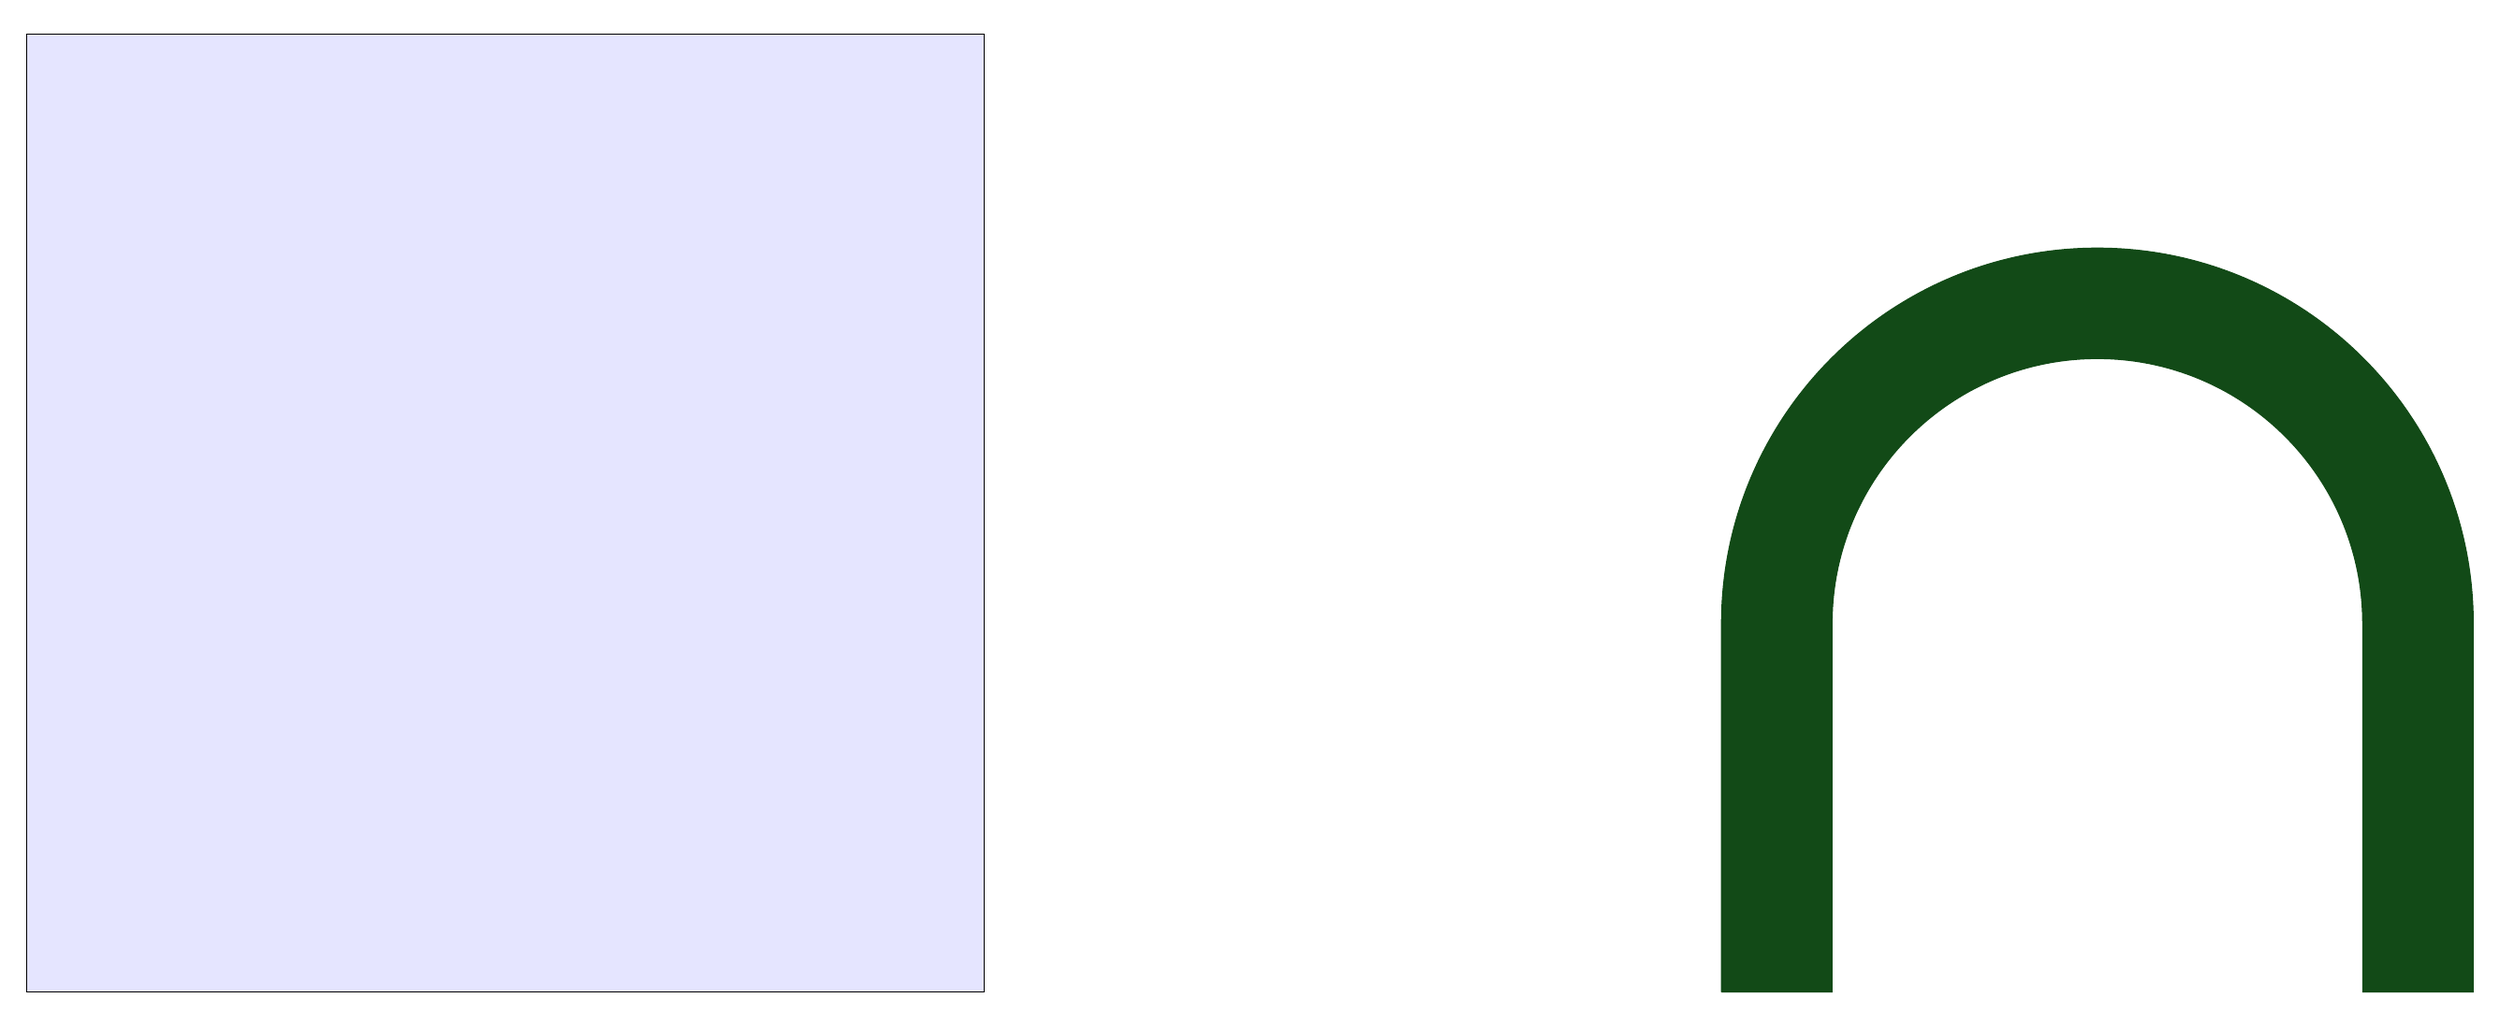
\begin{tikzpicture}

    % First left. Rectable is 130px.
    \path[draw,fill=blue!10] (0,0) -- ++(13.0,0) node (top) {} -- ++(0,-13.0)
        node (bottom){} -- ++(-13.0,0) -- cycle;

    % n 
        \draw[fill=ncbsgreen,draw=ncbsgreen] ($(bottom)+(10.0,0)$) -- ++(1.5,0) -- ++(0,5) 
        arc[radius=3.6, start angle=180, end angle=0] 
            -- ++(0,-5) -- ++(1.5,0) -- ++(0,5)
        arc[radius=5.1, start angle=0, end angle=180] 
            -- ++(0,-5);
            ;

\end{tikzpicture}
\end{document}

